\documentclass[accentcolor=tud9c,colorbacktitle,inverttitle,landscape,german,presentation,t]{tudbeamer}
\usepackage{amstext}
\usepackage{amsmath}
\usepackage{graphicx}
\usepackage{multicol}
\usepackage{mathtools}
\usepackage{subfigure}
\usepackage[ngerman,english]{babel}
\usepackage[utf8]{inputenc}
\usepackage{colortbl}
\usepackage{adjustbox}

\begin{document}


\title{\"Ubung 10 - Gruppe 142} 
\subtitle{Visual Computing - X3D – 3D in HTML} 

\author[Johannes Beck, Christian Eilers, Robin Menzenbach, Martin Steinborn]{Johannes Beck, Christian Eilers, Robin Menzenbach, Martin Steinborn}


\date{\today}

\begin{titleframe}
\end{titleframe}

\section{Aufgabe 1}
	\begin{frame}
		\frametitle{Aufgabe 1: Rendering}
		%Welche Informationen müssen für das Rendering einer 3D-Szene gegeben sein? 
		%TODO:Nennen Sie zusätzlich zu jedem Punkt ein Beispiel, welches nicht in der Vorlesung vorkam.
		\begin{itemize}
			\item Objekt-Geometrie, z.B.: Fenster, Torbögen
			\item Transformationen, z.B.: Duplizieren, Stapeln von gleichen Blöcken
			\item Materialien, z.B.: Bruchstellen, Veränderungen durch äußere Einflüsse
			\item Kameras, z.B.: Kamerafahrten
			\item Lichter, z.B.: Lichtbrechung im Fenster / Flüssigkeiten
			\item spezial-Effekte, z.B.: Feuer, Explosionen
		\end{itemize}
	\end{frame}

\section{Aufgabe 2}
\begin{frame}
	\frametitle{Aufgabe 2: X3D-Dokument}
	%Wie ist es möglich, in einem X3D-Dokument bestimmte Elemente mehrfach zu zeichnen, ohne diese mehrfach zu definieren?
	In einem X3D-Dokument ist es möglich bestimmte Elemente mehrfach zu zeichen, ohne sie mehrfach zu definieren, indem man innerhalb einer Gruppierung mehrere Transformationen einfügt, welche alle auf dieselben Objektdaten verweisen. So existiert ein Objekt, z.B. ein Rad nur einmalig, und es wird über 4 verschiedene Transformationen an den Achsen des Autos dargestellt.
\end{frame}

\section{Aufgabe 3}
\begin{frame}
	\frametitle{Aufgabe 3: Szenengraph-Standards}
	%TODO:Welche bekannten Szenengraph-Standards gibt es noch neben X3DOM? Nennen Sie mind. zwei und beschreiben Sie diese kurz.
	% Quelle: Skript und Wikipedia
			\begin{itemize}
			\item PHIGS oder Programmer’s Hierarchical Interactive Graphics System - Ist bis heute der ISO standart 9592 für Computergrafik. Es unterstützt unter anderem Punkte, Linien, gefüllte Polygone Transformationen, Perspektiven und Ebenen.
			\item VRML - Erstes Konzept für VR im Web und ist stark an OpenInventor angelehnt, ist aber deklarativ. Beherrscht 3D Geometrien, Ausleuchtung, Animation und Interaktion. Wird in Echtzeit generiert somit fallen Spiegelungen und Schattenwurf aus.
			\item X3D - Extensible 3D basiert auf XML und ist der Nachfolger des VRML - Standards. Es erlaubt neben XML auch Binary XML und VRML und bietet Profile für weitere Anwendugsfälle. Wird vom WWW Consortium empfohlen.
		\end{itemize}
\end{frame}

\section{Aufgabe 4}
\begin{frame}
	\frametitle{Aufgabe 4: Szenengraph – Hands on}
	%TODO:Erstellen Sie aus dem folgenden Bild einen Szenegraphen. Dieser sollte mindestens 6	Gruppierungsknoten enthalten. Enthält Ihr Graph bereits 6 Gruppierungsknoten, stellt aber nicht alle Details des Bildes dar, dann führt das nicht zu Punktabzug. Zeichnen Sie für einen Gruppierungsknoten beispielhaft die Transformations- und Objektknoten
	\centering
	\includegraphics[height=1\textheight]{aufg4.png}
\end{frame}

\section{Aufgabe 5}
\begin{frame}
	\frametitle{Aufgabe 5: Praktikum}
	%TODO:Erstellen Sie gemäß den folgenden Punkten eine X3DOM-Szene. Erstellen sie dazu eine einzige	HTML-Datei für ihr Markup und geben Sie diese separat ab.	Fertigen Sie ein Bild Ihrer Szene an und fügen sie es Ihrer Präsentation hinzu sowie eine Szene,die zunächst nichts bis auf eine Box in einer expliziten Farbe ihrer Wahl, platziert im Ursprung,enthält.	Färben Sie die eben erstellte Box grün.	Fügen Sie drei weitere Boxen hinzu und färben sie diese blau. Platzieren Sie diese Boxen links,rechts und oberhalb der bereits existierenden grünen Box.
	Die Bilder zeigen die Schrittweise entwicklung der geforderten Szene. Im ersten Bild wurde eine Box im Koordinatenzentrum in der Farbe gelb erstellt. Diese wurde dann wie im zweiten Bild zu sehen ist grün gefärbt. Als letztes wurden links rechts und oberhalb der grünen Box noch blaue Boxen ergänzt. Dies ist im dritten Bild zu sehen.\\
	
	\centering
	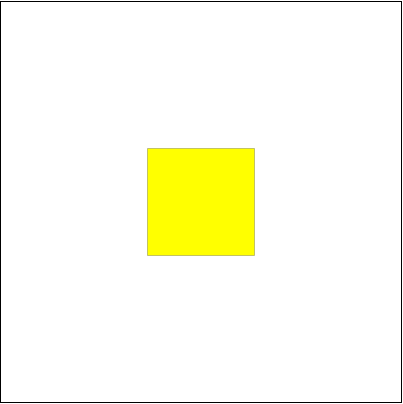
\includegraphics[width=0.25\linewidth]{task5_1.png}
	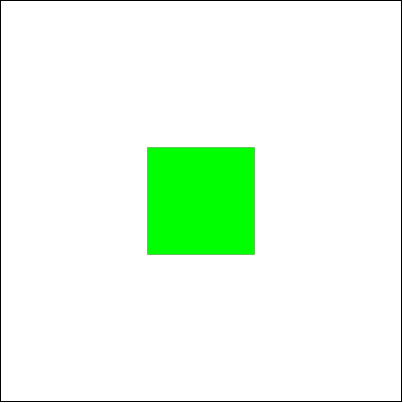
\includegraphics[width=0.25\linewidth]{task5_2.png}
	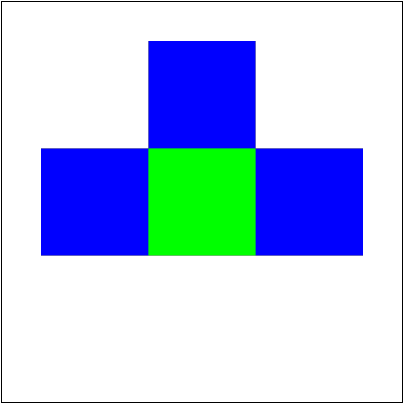
\includegraphics[width=0.25\linewidth]{task5_3.png}

	

\end{frame}
\end{document}
